
\paragraph{DELETE /:lang/user/:userId}
\begin{itemize}
\item \textbf{Successo}: \\
Questo scenario rappresenta il successo di una richiesta di eliminazione account che impone, come vincolo per poter essere effettuata, che l'utente sia autenticato al sistema.  
In questo caso il modulo \texttt{UserManagementController} invia \texttt{next()} per indicare il successo dell'operazione e successivamente verrà effettuata la logout() per completare interamente l'operazione.
\label{Procedura di eliminazione account}
\begin{figure}[ht]
	\centering
	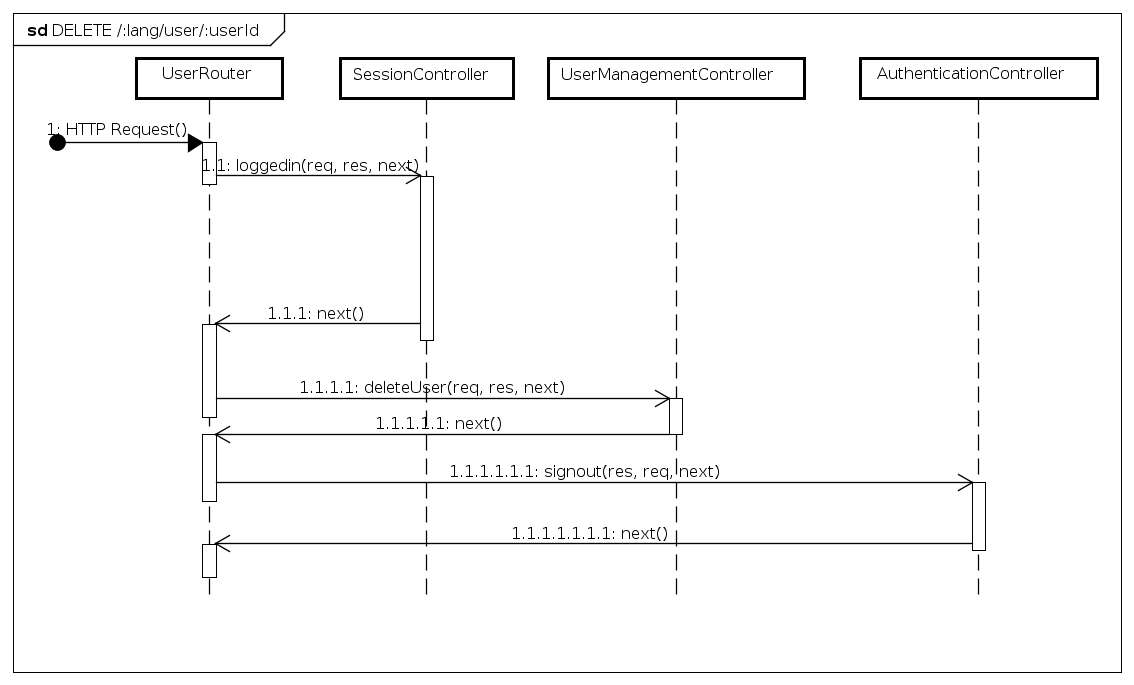
\includegraphics[scale=0.40]{UML/DiagrammiDiSequenza/Back-end/DELETE_LangUserUseridSuccess.png}
	\caption{DELETE /:lang/user/:userId}
\end{figure}
\FloatBarrier

\item \textbf{Fallimento}: \\
Quando viene effettuata una richiesta di eliminazione account sollevando un errore. Tale scenario rappresenta il fallimento di una richiesta di eliminazione account che impone, come vincolo per poter essere effettuata, che l'utente sia autenticato al sistema. In questo caso il modulo \texttt{UserManagementController} invia \texttt{next(error)} per il fallimento di tale vincolo al router il quale avrà compito di reinstradarlo (indirizzandolo verso \texttt{ErrorHandler}).

\label{Fallimento della procedura di eliminazione account}
\begin{figure}[ht]
	\centering
	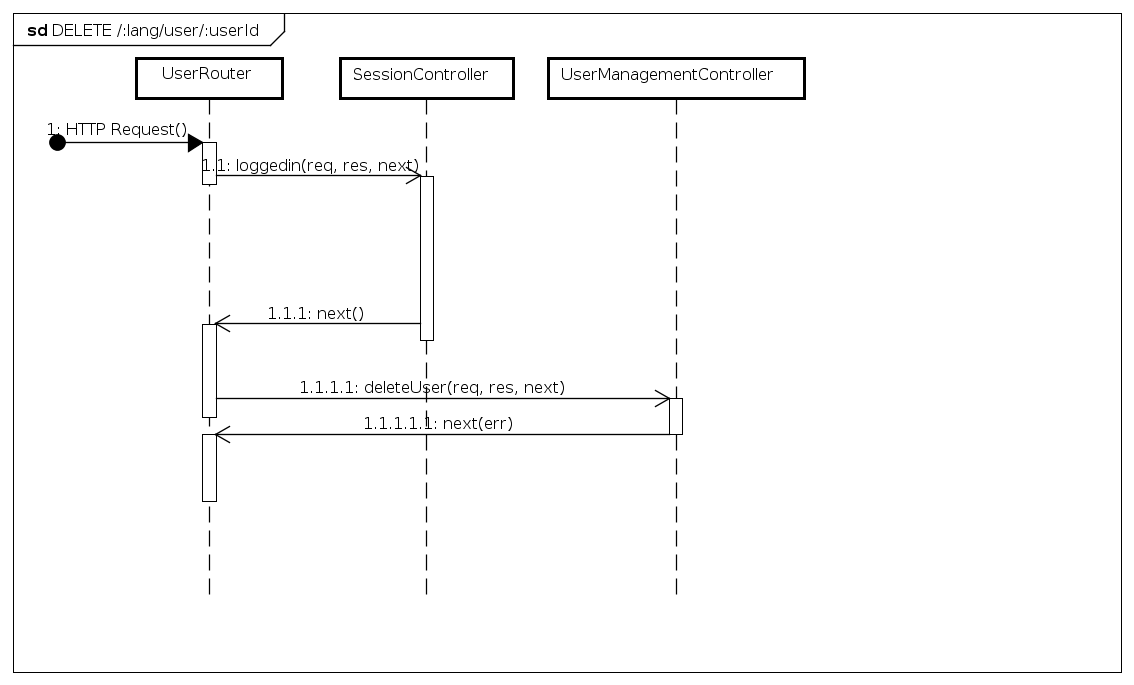
\includegraphics[scale=0.40]{UML/DiagrammiDiSequenza/Back-end/DELETE_LangUserUseridFailure.png}
	\caption{DELETE /:lang/user/:userId}
\end{figure}

\FloatBarrier
\end{itemize}

\paragraph{GET /:lang/user/:userId}
\begin{itemize}
\item \textbf{Successo}:\\
Questo scenario rappresenta il successo di una richiesta di visualizzazione dei dati dell'utente che impone, come vincolo per poter essere effettuata, che l'utente sia autenticato al sistema.  
In questo caso il modulo \texttt{UserManagementController} invia \texttt{next()} al router per indicare il successo dell'operazione.

\label{Procedura di visualizzazione dati utente}
\begin{figure}[ht]
	\centering
	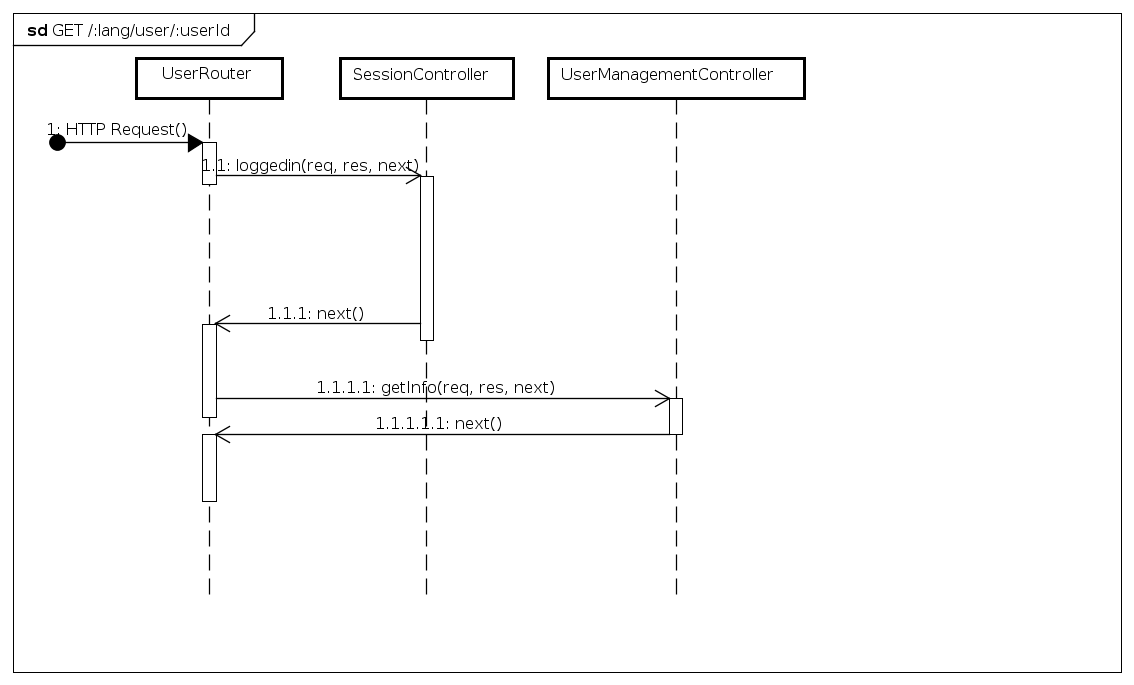
\includegraphics[scale=0.40]{UML/DiagrammiDiSequenza/Back-end/GET_LangUserUserIdSuccess.png}
	\caption{GET /:lang/user/:userId}
\end{figure}

\FloatBarrier

\item \textbf{Fallimento}:
\\
Quando viene effettuata una richiesta di visualizzazione dei dati dell'utente sollevando un errore. Tale scenario rappresenta il fallimento di una richiesta di visualizzzione dei dati dell'utente che impone, come vincolo per poter essere effettuata, che l'utente sia autenticato al sistema. In questo caso il modulo \texttt{UserManagementController} invia \texttt{next(error)} per il fallimento di tale vincolo al router il quale avrà compito di reinstradarlo (indirizzandolo verso \texttt{ErrorHandler}).

\label{Fallimento della procedura di visualizzazione dati utente}
\begin{figure}[ht]
	\centering
	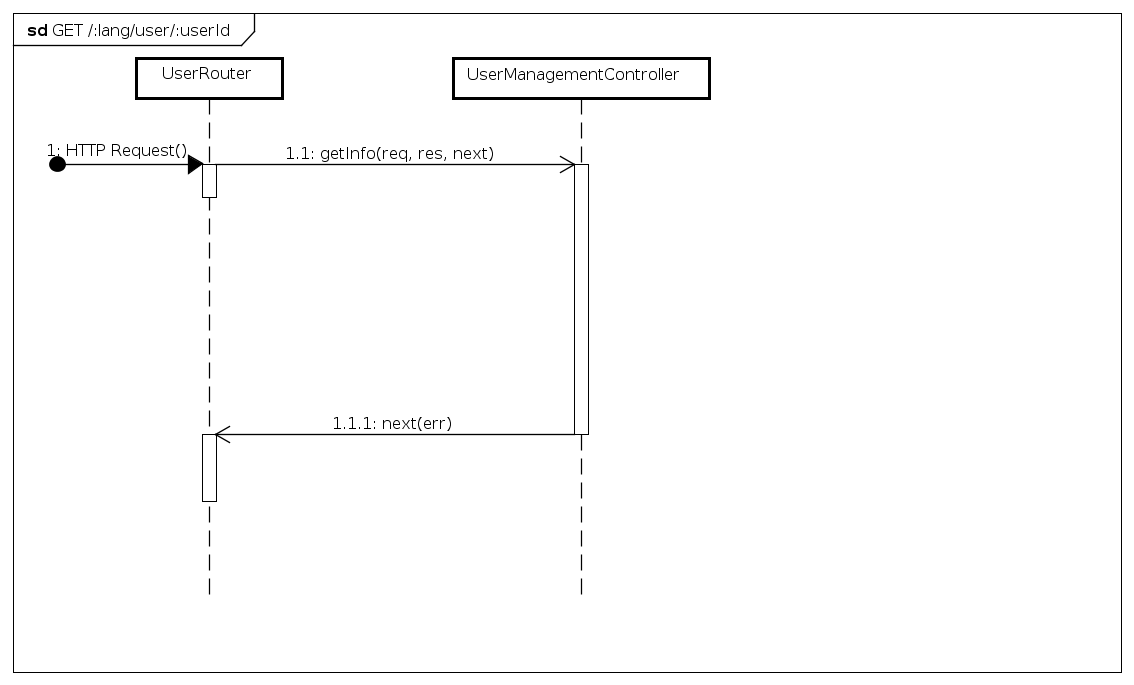
\includegraphics[scale=0.40]{UML/DiagrammiDiSequenza/Back-end/GET_LangUserUseridFailure.png}
	\caption{GET /:lang/user/:userId}
\end{figure}

\FloatBarrier
\end{itemize}

\paragraph{PUT /:lang/user/:userId}
\begin{itemize}
\item \textbf{Successo}:
\\
Questo scenario rappresenta il successo di una richiesta di modifica dei dati dell'utente che impone, come vincolo per poter essere effettuata, che l'utente sia autenticato al sistema.  
In questo caso il modulo \texttt{UserManagementController} invia \texttt{next()} al router per indicare il successo dell'operazione.
\label{Procedura di modifica dati utente}
\begin{figure}[ht]
	\centering
	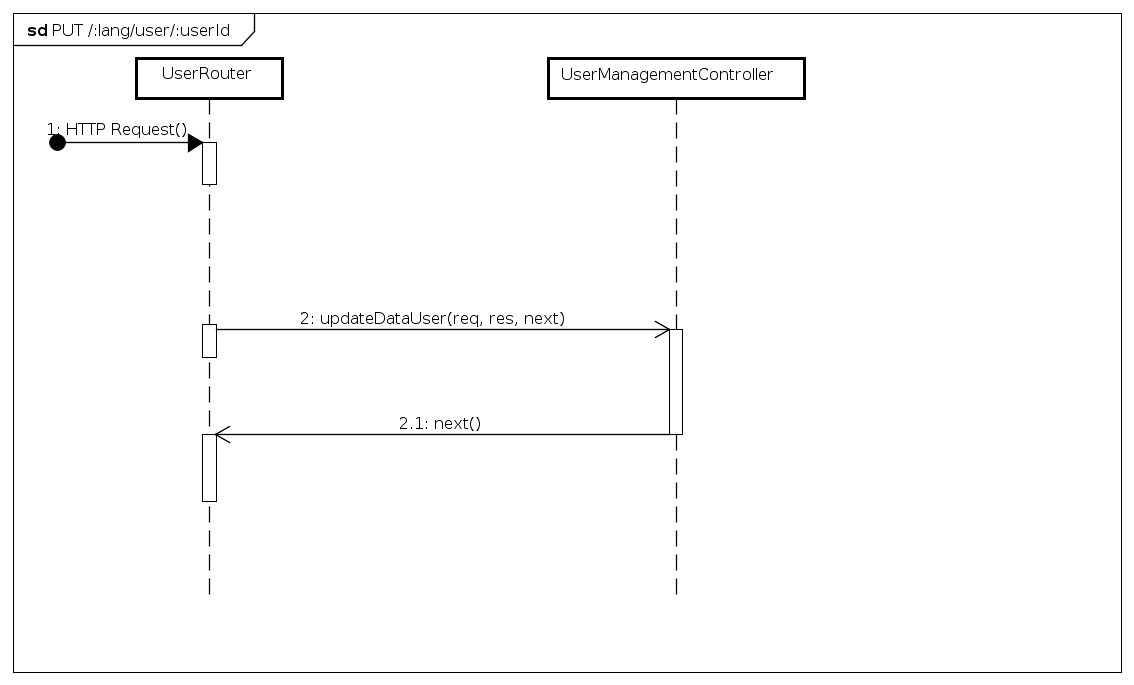
\includegraphics[scale=0.40]{UML/DiagrammiDiSequenza/Back-end/PUT_LangUserUseridSuccess.png}
	\caption{PUT /:lang/user/:userId}
\end{figure}
\FloatBarrier

\item \textbf{Fallimento}:
\\
Quando viene effettuata una richiesta di modifica dei dati dell'utente sollevando un errore. Tale scenario rappresenta il fallimento di una richiesta di modifica dei dati dell'utente che impone, come vincolo per poter essere effettuata, che l'utente sia autenticato al sistema. In questo caso il modulo \texttt{UserManagementController} invia \texttt{next(error)} per il fallimento di tale vincolo al router il quale avrà compito di reinstradarlo (indirizzandolo verso \texttt{ErrorHandler}).
\label{Fallimento della procedura di modifica dati utente}
\begin{figure}[ht]
	\centering
	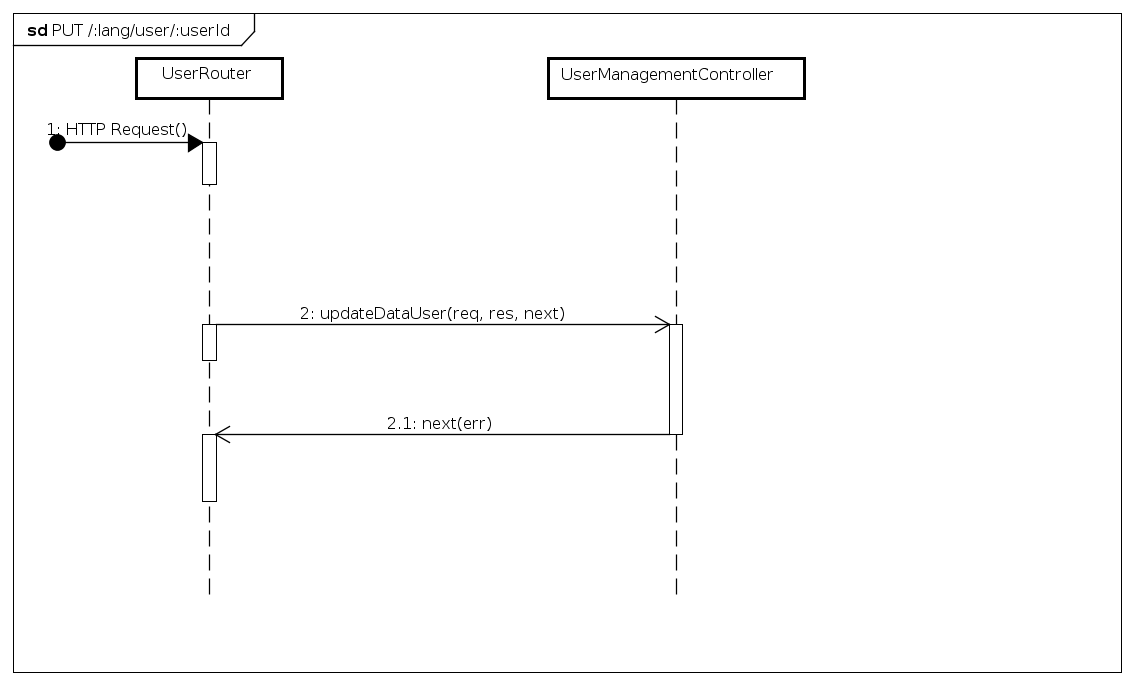
\includegraphics[scale=0.40]{UML/DiagrammiDiSequenza/Back-end/PUT_LangUserUseridFailure.png}
	
	\caption{PUT /:lang/user/:userId}
\end{figure}
\FloatBarrier
\end{itemize}

\paragraph{PUT /:lang/user/:userId/privacy}
\begin{itemize}
\item \textbf{Successo}
\\
Questo scenario rappresenta il successo di una richiesta di modifica della passwprd dell'utente che impone, come vincolo per poter essere effettuata, che l'utente sia autenticato al sistema.  
In questo caso il modulo \texttt{UserManagementController} invia \texttt{next()} al router per indicare il successo dell'operazione.

\label{Procedura di modifica password}
\begin{figure}[ht]
	\centering
	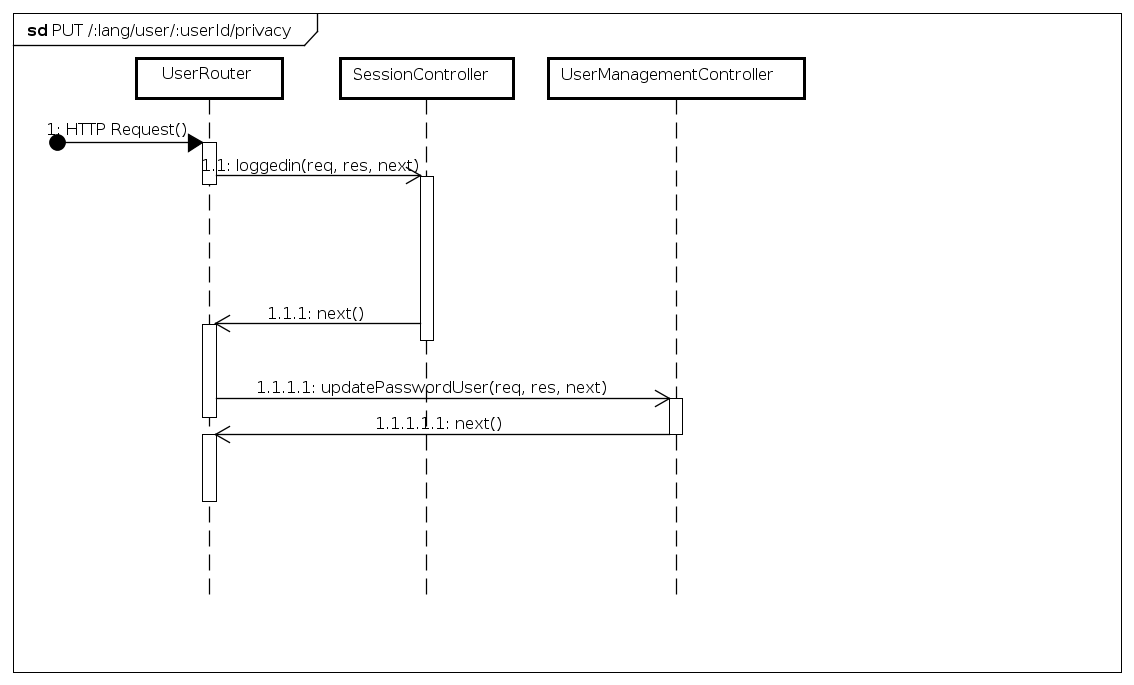
\includegraphics[scale=0.40]{UML/DiagrammiDiSequenza/Back-end/PUT_LangUserUserIdPrivacySuccess.png}
	\caption{PUT /:lang/user/:userId/privacy}
\end{figure}
\FloatBarrier
\item \textbf{Fallimento}
\\
Quando viene effettuata una richiesta di modifica della password dell'utente sollevando un errore. Tale scenario rappresenta il fallimento di una richiesta di modifica della password dell'utente che impone, come vincolo per poter essere effettuata, che l'utente sia autenticato al sistema. In questo caso il modulo \texttt{UserManagementController} invia \texttt{next(error)} per il fallimento di tale vincolo al router il quale avrà compito di reinstradarlo (indirizzandolo verso \texttt{ErrorHandler}).



\label{Fallimento della procedura di modifica password}
\begin{figure}[ht]
	\centering
	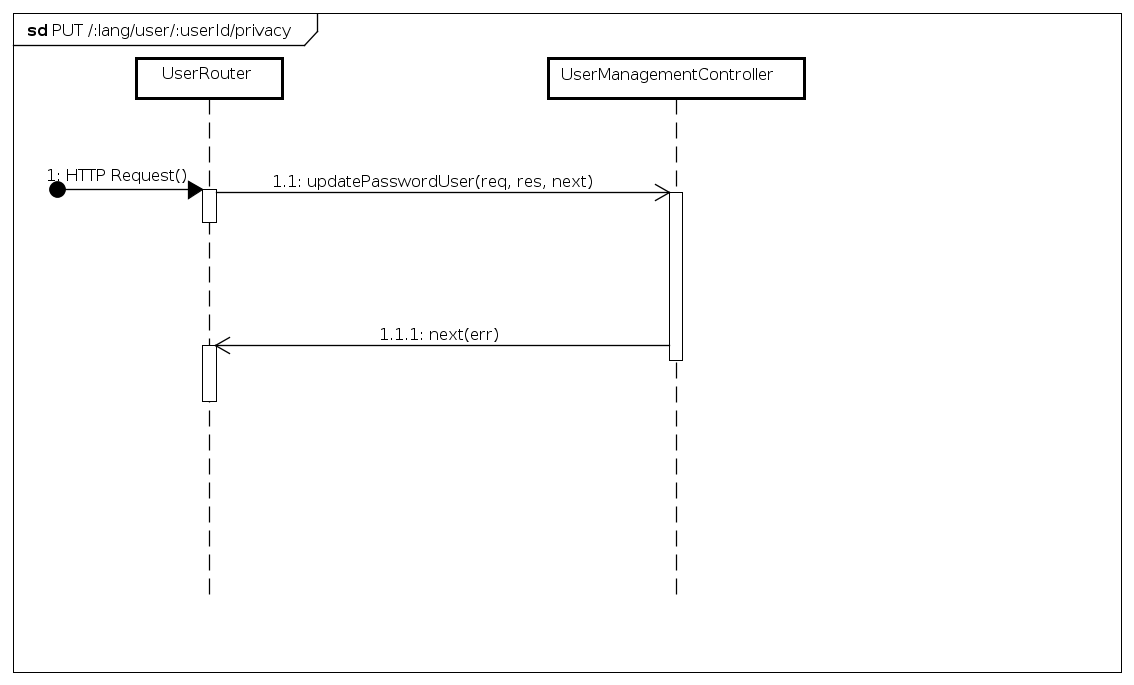
\includegraphics[scale=0.40]{UML/DiagrammiDiSequenza/Back-end/PUT_LangUserUserIdPrivacyFailure.png}	
	\caption{PUT /:lang/user/:userId/privacy}
\end{figure}
\FloatBarrier
\end{itemize}


\paragraph{GET /:lang/user/:userId/statistics}
\begin{itemize}
\item \textbf{Successo}:
\\
Questo scenario rappresenta il successo di una richiesta di modifica delle statistiche  dell'utente che impone, come vincolo per poter essere effettuata, che l'utente sia autenticato al sistema.  
In questo caso il modulo \texttt{UserManagementController} invia \texttt{next()} al router per indicare il successo dell'operazione.

\label{Procedura di visualizzazione delle statistiche}
\begin{figure}[ht]
	\centering
	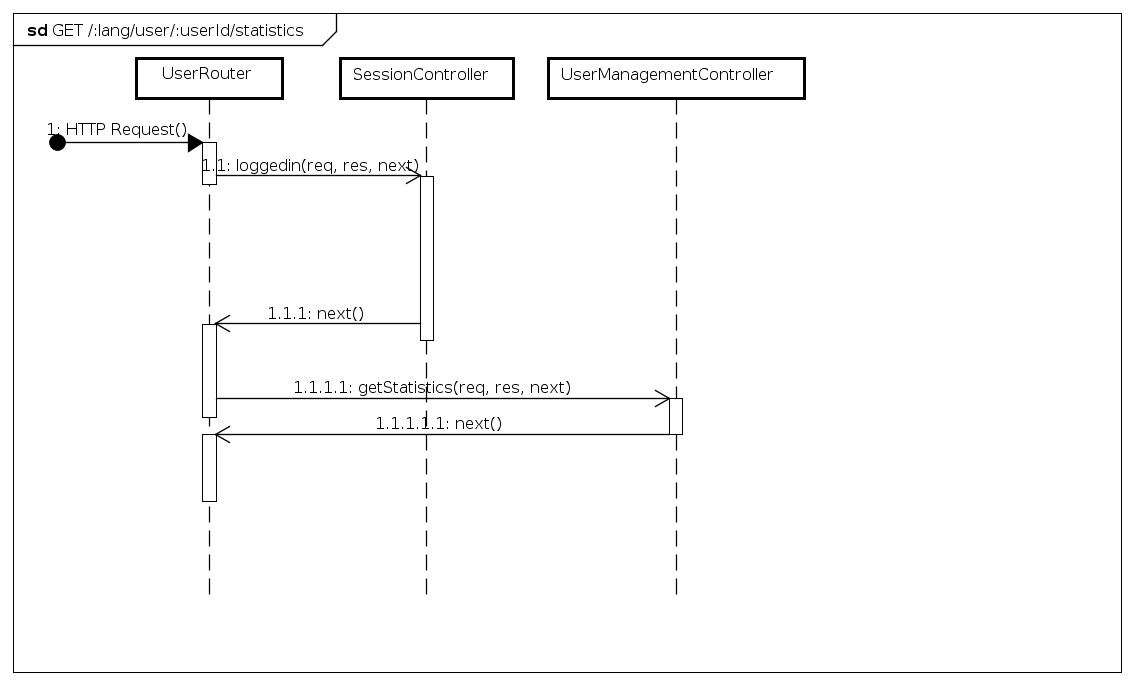
\includegraphics[scale=0.40]{UML/DiagrammiDiSequenza/Back-end/GET_LangUserUserIdStatisticsSuccess.png}
	\caption{GET /:lang/user/:userId/statistics}
\end{figure}
\FloatBarrier
\item \textbf{Fallimento}
\\
Quando viene effettuata una richiesta di visualizzazione delle statistiche dell'utente sollevando un errore. Tale scenario rappresenta il fallimento di una richiesta di visualizzazione delle statistiche dell'utente che impone, come vincolo per poter essere effettuata, che l'utente sia autenticato al sistema. In questo caso il modulo \texttt{UserManagementController} invia \texttt{next(error)} per il fallimento di tale vincolo al router il quale avrà compito di reinstradarlo (indirizzandolo verso \texttt{ErrorHandler}).

\label{Fallimento della procedura di visualizzazione delle statistiche}
\begin{figure}[ht]
	\centering
	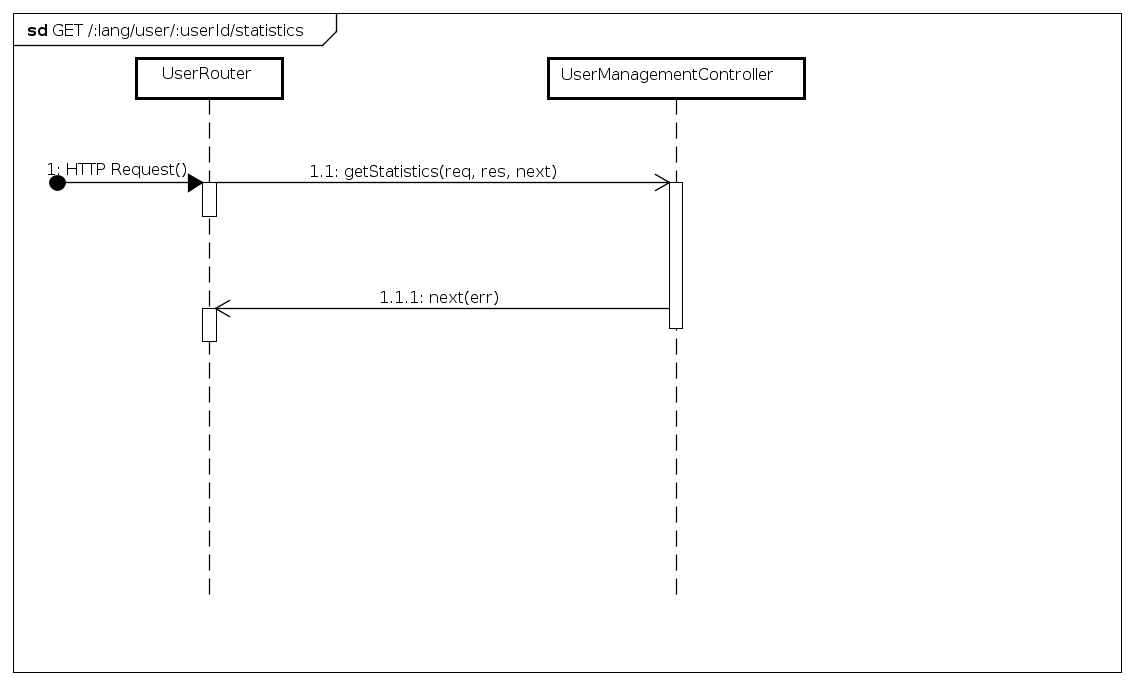
\includegraphics[scale=0.40]{UML/DiagrammiDiSequenza/Back-end/GET_LangUserUserIdStatisticsFailure.png}
	\caption{GET /:lang/user/:userId/statistics}
\end{figure}
\FloatBarrier
\end{itemize}

\paragraph{GET /:lang/user/:userId/statistics/summary/}
\begin{itemize}
\item \textbf{Successo}:
\\
Questo scenario rappresenta il successo di una richiesta di visualizzazione della cronologia dei questionari svolti dall'utente che impone, come vincolo per poter essere effettuata, che l'utente sia autenticato al sistema.  
In questo caso il modulo \texttt{UserManagementController} invia \texttt{next()} al router per indicare il successo dell'operazione.
\label{Procedura di visualizzazione della cronologia dei questionari svolti}
\begin{figure}[ht]
	\centering
	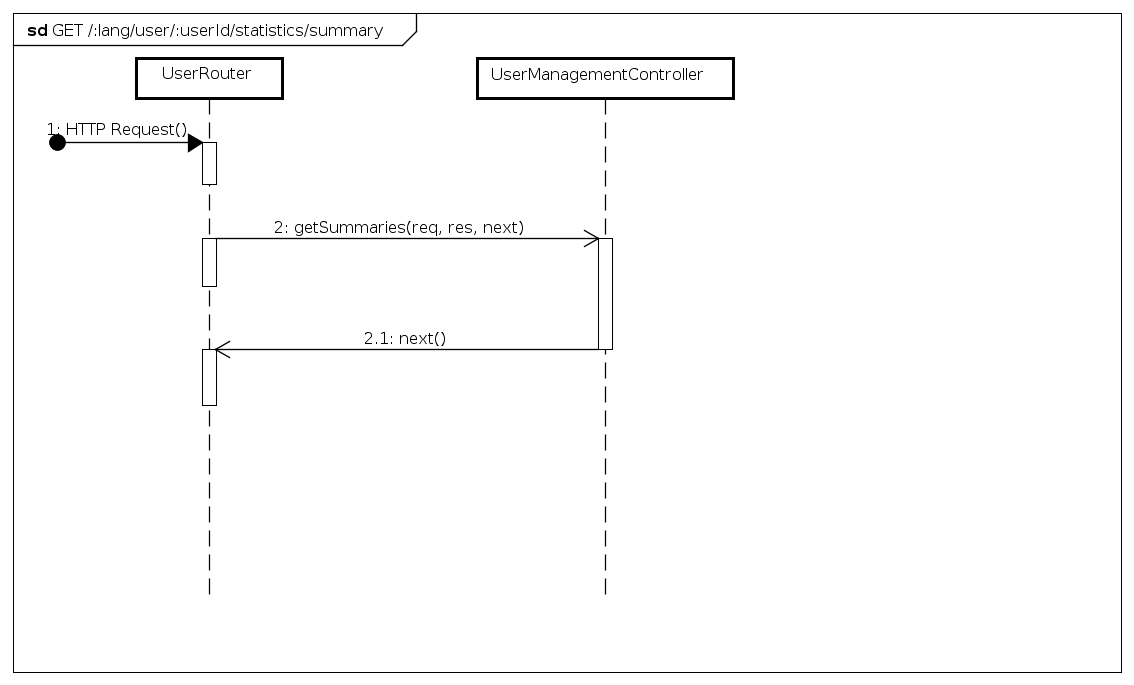
\includegraphics[scale=0.40]{UML/DiagrammiDiSequenza/Back-end/GET_LangUserUserIdStatisticsSummarySuccess.png}
	\caption{GET /:lang/user/:userId/statistics/summary}
\end{figure}
\FloatBarrier
\item \textbf{Fallimento}:
\\
Quando viene effettuata una richiesta di visualizzazione della cronologia dei questionari svolti dall'utente sollevando un errore. Tale scenario rappresenta il fallimento di una richiesta di visualizzazione della cronologia dei questionari svolti dall'utente che impone, come vincolo per poter essere effettuata, che l'utente sia autenticato al sistema. In questo caso il modulo \texttt{UserManagementController} invia \texttt{next(error)} per il fallimento di tale vincolo al router il quale avrà compito di reinstradarlo (indirizzandolo verso \texttt{ErrorHandler}).
\label{Fallimento della procedura di visualizzazione della cronologia dei questionari svolti}
\begin{figure}[ht]
	\centering
	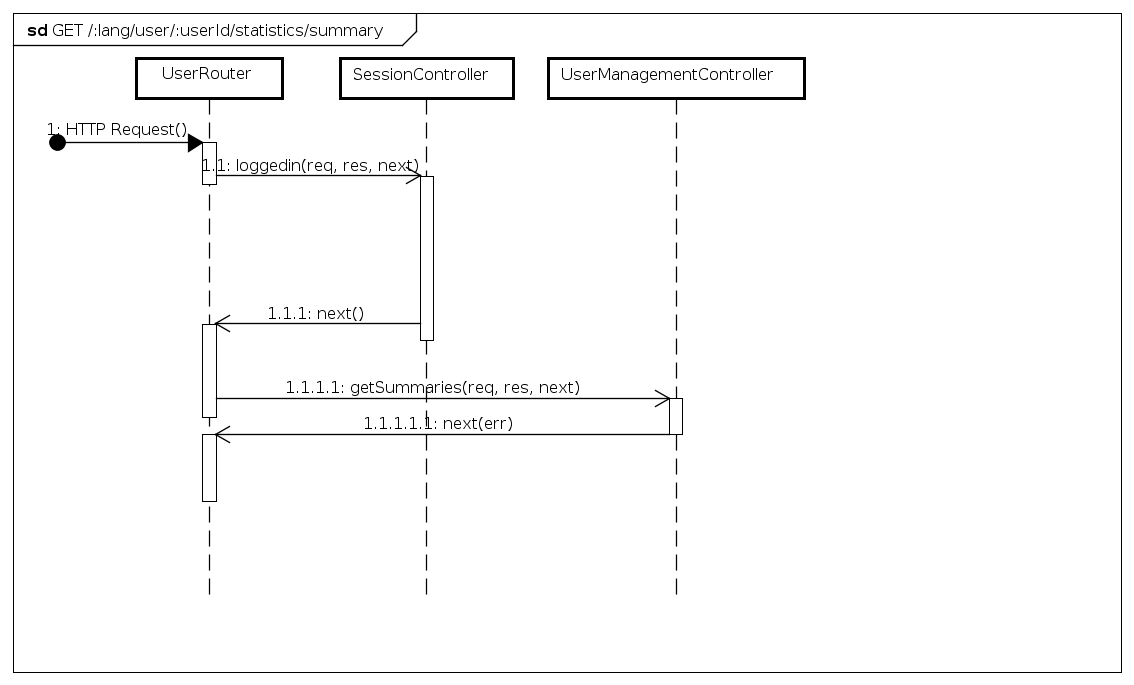
\includegraphics[scale=0.40]{UML/DiagrammiDiSequenza/Back-end/GET_LangUserUserIdStatisticsSummaryFailure.png}
	\caption{GET /:lang/user/:userId/statistics/summary}
\end{figure}
\FloatBarrier

\end{itemize}

\paragraph{GET /:lang/user/:userId/statistics/summary/:summaryId}
\begin{itemize}
\item \textbf{Successo}
\\
Questo scenario rappresenta il successo di una richiesta di visualizzazione del riepilogo di un particolare questionario svolto dall'utente che impone, come vincolo per poter essere effettuata, che l'utente sia autenticato al sistema.  
In questo caso il modulo \texttt{UserManagementController} invia \texttt{next()} al router per indicare il successo dell'operazione.
\label{Procedura di visualizzazione del riepilogo di un particolare questionario svolto}
\begin{figure}[ht]
	\centering
	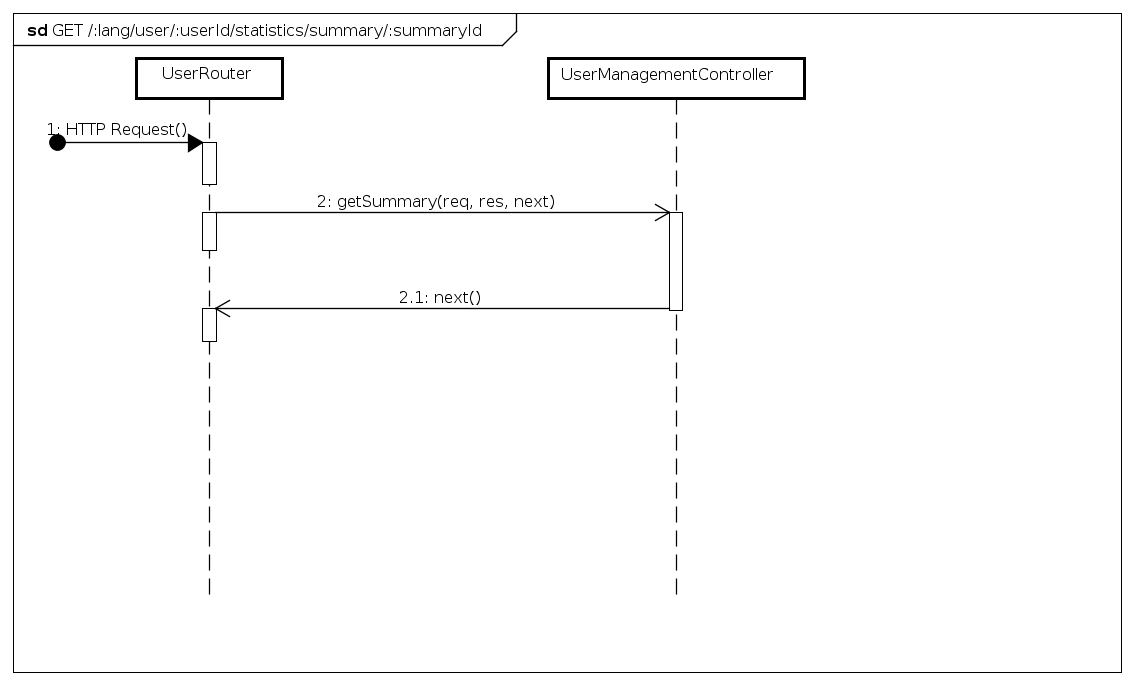
\includegraphics[scale=0.40]{UML/DiagrammiDiSequenza/Back-end/GET_LangUserUserIdStatisticsSummarySummaryIdSuccess.png}
	\caption{GET /:lang/user/:userId/statistics/summary/:summaryId}
\end{figure}
\FloatBarrier
\item \textbf{Fallimento}:
\\
Quando viene effettuata una richiesta di visualizzazione del riepilogo di un particolare questionario svolto dall'utente sollevando un errore. Tale scenario rappresenta il fallimento di una richiesta di visualizzazione del riepilogo di un particolare questionario svolto dall'utente che impone, come vincolo per poter essere effettuata, che l'utente sia autenticato al sistema. In questo caso il modulo \texttt{UserManagementController} invia \texttt{next(error)} per il fallimento di tale vincolo al router il quale avrà compito di reinstradarlo (indirizzandolo verso \texttt{ErrorHandler}).
\label{Fallimento della procedura di visualizzazione del riepilogo di un particolare questionario svolto}
\begin{figure}[ht]
	\centering
	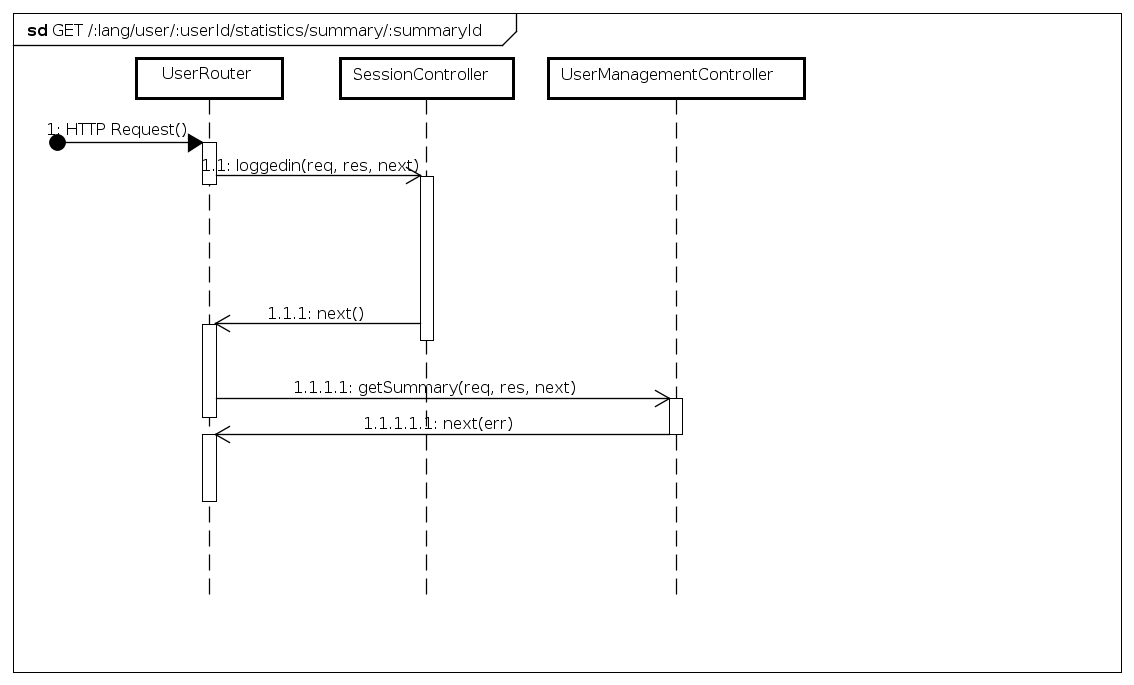
\includegraphics[scale=0.40]{UML/DiagrammiDiSequenza/Back-end/GET_LangUserUserIdStatisticsSummarySummaryIdFailure.png}
	\caption{GET /:lang/user/:userId/statistics/summary/summaryId}
\end{figure}
\FloatBarrier
\end{itemize}



